\documentclass[border=4pt]{standalone}

\usepackage{mathpazo}
\usepackage{pgfplots}
\newcommand{\num}{pi}
\pgfplotsset{compat=1.8}
 % define the plot style and the axis style
\tikzset{elegant/.style={smooth,thick,samples=500,magenta}} %samples设置采样点数量

\begin{document}

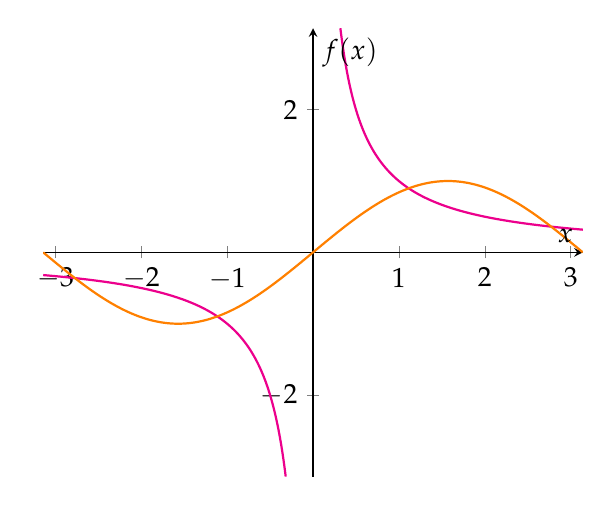
\begin{tikzpicture}
    % the axis environment 
    \begin{axis}[axis x line=middle,
                 axis y line=middle,
                 ylabel=$f(x)$,
                 xlabel=$x$]
        \addplot[elegant,domain=-\num:-1/\num]{1/x};
        \addplot[elegant,domain=1/\num:\num]{1/x};
        \addplot[elegant,orange,domain=-\num:\num]{sin(deg(x))};
    \end{axis}
\end{tikzpicture}

\end{document}